\chapter{JVM}
% \section*{25 - Settembre}
\section{Runtime System}
Every language defines and \textbf{execution model}, which is (partially) implemented by a \textbf{runtime system},
providing runtime \textbf{support} needed by both \textit{compiled} and \textit{interpreted} programs.
\parskip = \baselineskip

A \textbf{Runtime system} includes (eventually):
\begin{itemize}
    \item Code:
    \begin{itemize}
        \item in the executing program generated by the compiler
        \item running in other threads/processes ]
    \end{itemize}
    \item Language libraries
    \item Operating system functionalities
    \item The interpreter/virtual machine itself
\end{itemize}


\textbf{Runtime support} can be needed for various reasons:
\begin{itemize}
    \item %Memory management
    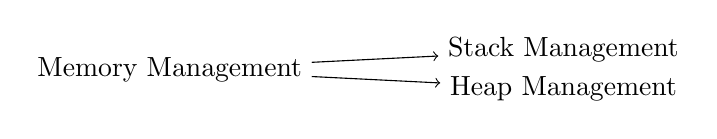
\begin{tikzpicture}
        \node[draw=white,align=left] (A) at (0,0.25) {Memory Management};
        \node[draw=white,align=left] (B) at (5,0.5) {Stack Management};
        \node[draw=white,align=left] (C) at (5,0) {Heap Management};

        \path [->] (A) edge node[left] {} (B);
        \path [->] (A) edge node[left] {} (C);
    \end{tikzpicture}
    \item 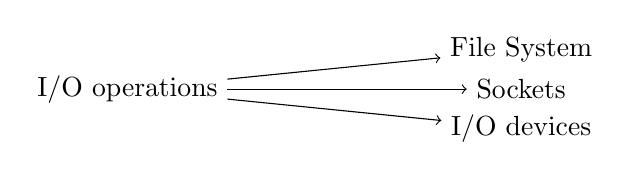
\begin{tikzpicture}
        \node[draw=white,align=left] (A) at (0,0.5) {I/O operations};
        \node[draw=white,align=left] (B) at (5,1) {File System};
        \node[draw=white,align=left] (C) at (5,0.5) {Sockets};
        \node[draw=white,align=left] (D) at (5,0) {I/O devices};

        \path [->] (A) edge node[left] {} (B);
        \path [->] (A) edge node[left] {} (C);
        \path [->] (A) edge node[left] {} (D);
    \end{tikzpicture}
    \item Intercation with runtime environment
    \item Parallel execution (threads/processes)
    \item Dynamic binding type checking
    \item Dynamic loading and linking of modules
    \item Debugging
    \item Code Generation for JIT compilation and optimization
    \item Verification and Monitoring
\end{itemize}

\subsection{JRE}
The \textbf{Java Runtime Environmnet} includes \textbf{JVM} and \textbf{JCL} (\textit{Java Class Library}).

\section{JVM}
\textbf{JVM} is an \textit{abstract} machine, defined by the documentation,
which \ul{\textit{omits implementation details}} on stuff like memory layout of runtime data area, garbage-collection, internal optimization, and even the representation of the \lstinline{null} constant.
The JVM specification, instead, defines precisely a machine indipendent \textit{``class file format''} that all JVM implementations must support;
it also imposes strong \textbf{synctatic} and \textbf{structural constraints} on the code in a class file.
\nl

The \textbf{JVM} is not \textit{register-based}, instead it is a \textit{multi-threaded \textbf{stack}\footnote{Not to be confused with the stack of activation records!} based machine}.
Id est the JVM pops intructions from the top of \textbf{operand stack} of the current frame, and pushes their result on the top of the \textbf{operand stack}. 
The \textbf{operand stack} is used to:
\begin{itemize}
    \item Pass arguments to functions
    \item Return results from a function
    \item Store intermediate values while evaluating expressions
    \item Store local variables
\end{itemize}
\begin{center}
    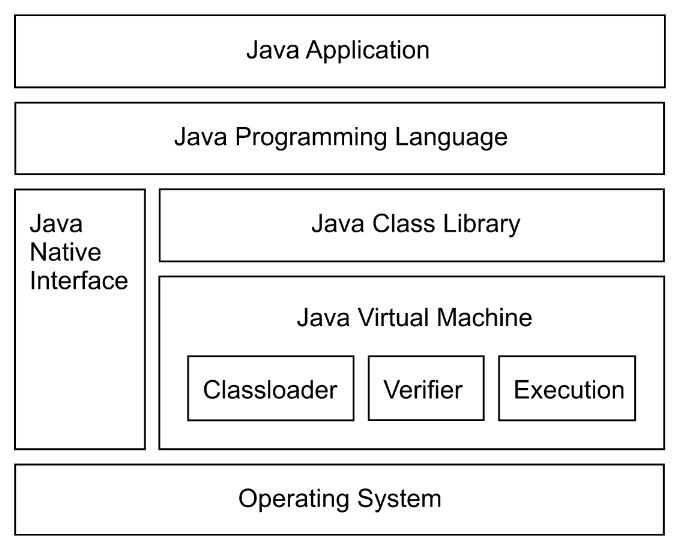
\includegraphics[width=0.4\textwidth]{images/Java_hierarchy.png}
\end{center}

\subsection{Data types}
\lstinline{.class} file are platform independent external representations, which are represented internally by the JVM using simpler data types, which are implementation dependent.
\begin{itemize}
    \item \textbf{Primitive types}
    \begin{itemize}
        \item Numerica integral
        \item Numeric floating point
        \item boolean (support only for arrays)
        \item internal (for exception handling)
    \end{itemize}
    \item \textbf{Reference types}
    \begin{itemize}
        \item Class types
        \item Array types
        \item Interface types
    \end{itemize}
    \item[] \note{No type information on local variables at runtime, there are only operand types specified by \textbf{opcodes} e.g. \lstinline{iadd, fadd,...}}
\end{itemize}

\subsection{Threads}
There are some runtime areas of the JVM related to a single thread, while others are shared among threads

\begin{center}
    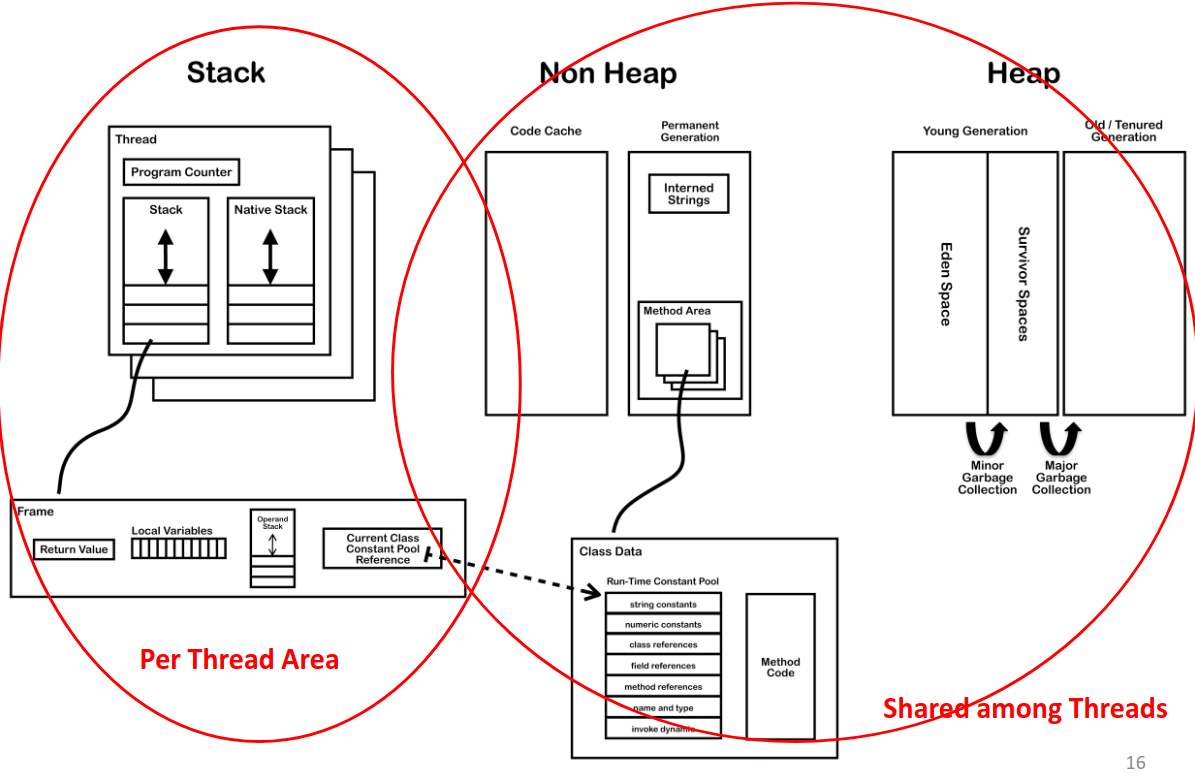
\includegraphics[width=0.6\textwidth]{images/JVM_Runtime_areas.png}
\end{center}
All Java Programs are multithreaded, since there is at least a \lstinline{main} thread running the user's program, and many \textbf{daemons}:
\begin{itemize}
    \item Garbage collector
    \item Signal Dispatching
    \item Compilation
    \item etc \dots
\end{itemize}
JVM doesn't pose strong implementation constraints by defining a precise abstract consistency model, including volatiles, allowing non-atomic longs and doubles, distinguishing working-memory and general store.


\subsection{per-thread Data Areas}
\begin{itemize}
    \item \textbf{pc} pointer to next instruction in \textit{method area}\\
    \textit{undefined }if current method is \textit{native}. When a native function is invoked, execution continues using the native stack. However, a native function, can invoke a Java method, in which case the pc is set to the first instruction of the invoked method, in Java stack.
    
    \item \textbf{Java stack}: stack of \textit{frames} (or \textit{activation records)}
    \item \textbf{Native stack}: used for invocation of natve functions through the \textit{Java Native Interface} (\textit{JNI})\\
    Native methods are written in languages like C or C++ and invoked from Java code using the Java Native Interface (JNI).\\
    They are used, for instance, by \texttt{java.lang.System}, \texttt{java.io.File}, \texttt{java.nio.channels.Selector}, and others. In general they are exploited for I/O operations, Thread management (thread creation may be performed at OS level), and networking (\texttt{java.net}).
\end{itemize}

\subsubsection{Frames}
{Considering the \textbf{structure} of \textbf{frames}, each one is created upon method invocation, and  is composed by:\ns
\begin{itemize}
    \item \textbf{Local Variable Array} (32 bits) containing:
    \begin{enumerate}
        \item Reference to \lstinline{this}
        \item Method parameters
        \item Local variables
    \end{enumerate}
    \item \textbf{Operand stack}
    \item Reference to \textbf{Constant Pool} of current class
\end{itemize}}

Differently from C/C++, where the \textbf{linking} phase is done before running an executable,
java computes linking \textbf{dynamically} at \textbf{runtime};
this is achieved using \textbf{symbolic} references, which can be resolved using \textit{static} (eager) or \textit{late} (lazy) resolution.\\
Since the execution of a Java program must \textbf{not} depend on the JVM implementation, the JVM always behaves as if the implementation implies \textit{lazy} resolution, 
even if the actual implementation provides static resolution instead.

\subsection{Shared data areas}
\subsubsection{Heap}
\begin{itemize}
    \item Memory for objects and arrays
    \item No explicit deallocation, it is demanded to the garbage collection.
\end{itemize}

\subsubsection{Non-Heap}
Memory for objects never deallocated
\begin{itemize}
    \item Method area
    \item Interned strings
    \item Code cache for JIT
\end{itemize}

\textit{Just In Time} (JIT) compilation refers to profiling as ``hot'' code areas of bytecode which may be executed many times, and storing the compiled native code in a cache in the \textit{Non-heap} memory.

\subsubsection{Method-area}
Here \lstinline{class} files are loaded.
For each class a classloader reference and the following info from the \lstinline{class} file are stored:
\begin{itemize}
    \item Runtime Constant Pool
    \item Field data
    \item Method data
    \item Method code
\end{itemize}

\note{\texttt{Method area is \textit{shared} among threads}! Access to it must be \textit{\textbf{thread safe}}.}

This should a \textbf{permanent} area of the memory, but it may be \textbf{edited} when a new class is loaded or when a symbolic link is resolved by dynamic linking.


% \section*{26 - Settembre}
\subsubsection{Constant Pool}
Contains constants and symbolic references for dynamic binding.
It is possible to see the constant pool of a compiled \lstinline{.class} file using the command:
\begin{lstlisting}
javap -v name.class
\end{lstlisting}
Displaying something resembling to:
\begin{lstlisting}
   #1 = Methodref          #6.#14         // java/lang/Object."<init>":()V
   #2 = Fieldref           #15.#16        // java/lang/System.out:Ljava/io/PrintStream;
   #3 = String             #17            // Hello World
   #4 = Methodref          #18.#19        // java/io/PrintStream.println:(Ljava/lang/String;)V
   #5 = Class              #20            // com/baeldung/jvm/ConstantPool
   #6 = Class              #21            // java/lang/Object
   #7 = Utf8               <init>
   #8 = Utf8               ()V
   #9 = Utf8               Code
  #10 = Utf8               LineNumberTable
  #11 = Utf8               sayHello
  #12 = Utf8               SourceFile
\end{lstlisting}

\begin{paracol}{2}
    
    Similar to symbol table, but with more info: it contains constants and symbolic references used for
    dynamic binding, suitably tagged
    \begin{itemize}
        \item numeric literals (Integer, Float, Long, Double)
        \item string literals (Utf8)
        \item class references (Class)
        \item field references (Fieldref)
        \item method references (Mehodref, InterfaceMethodref, MethodHandle)
        \item signatures (NameAndType)
    \end{itemize}
    \note{Operands in bytecodes often are indexes in the
    constant pool}
    
    \switchcolumn

    \begin{figure}[htbp]
        \centering
        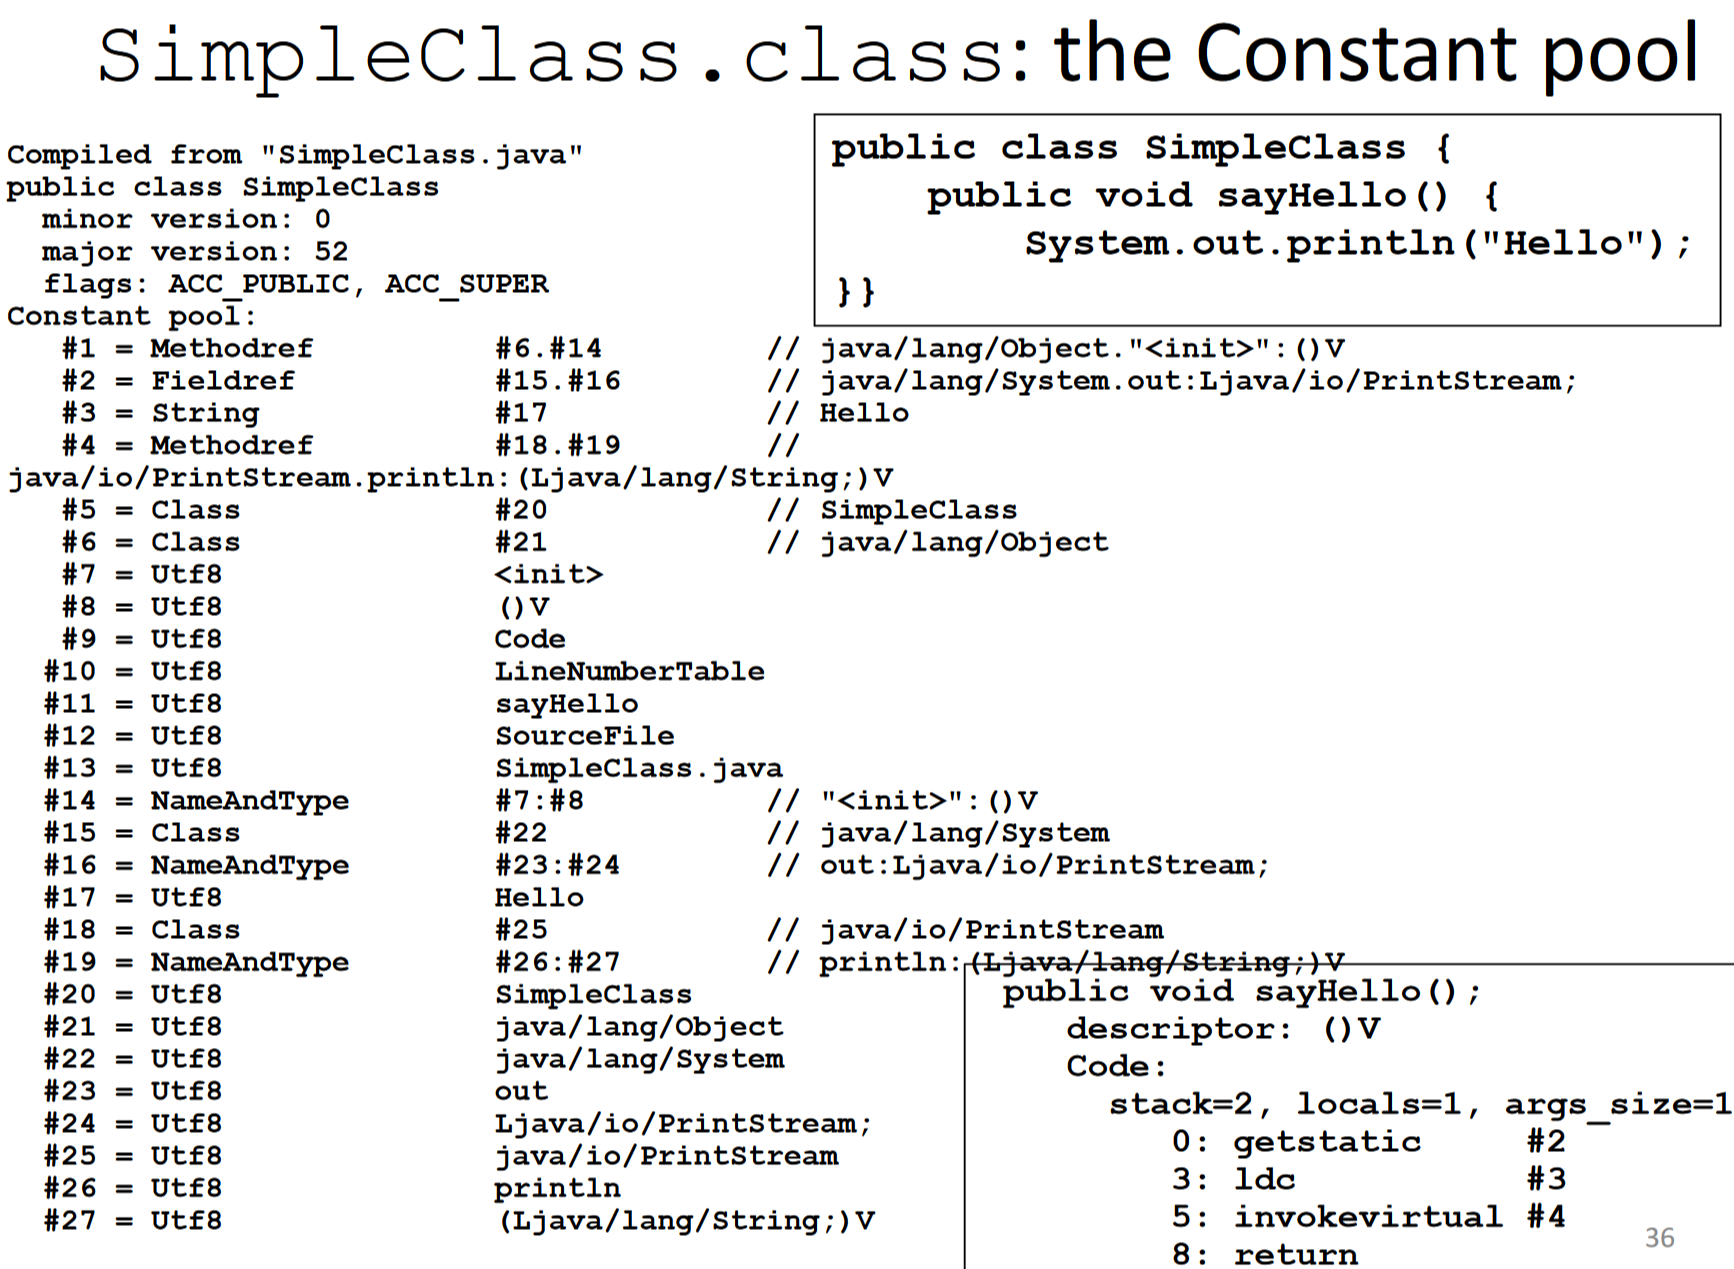
\includegraphics[width=0.9\columnwidth]{images/jvm_pool.png}
        \caption{Constant Pool example}
        \label{fig:jvm_pool}
    \end{figure}

\end{paracol}

Recall that \ul{variables are \textbf{not} here}.
\begin{itemize}
    \item \textbf{Local} variables and method \textbf{parameters} are in the \textbf{local variable array} of the current frame
    \item \textbf{Class} variables (\texttt{static} fields) are in the method area 
    \item \textbf{Instance} variables are in the heap as part of the object instance
\end{itemize}

\subsection{Loading}
\textbf{Loading} is finding the binary representation of a class or interface type with a given name and creating a class or interface from it.\\
Class (or Interface) $C$ creation is \textit{triggered} by other classes \textbf{referencing} $C$ or by methods (e.g. reflection\footnote{This contributes to the performance footprint of reflection, discussed later in Sec. \ref{sec:reflection_drawbacks}}).
If not previously loaded, \lst{loader.loadClass} is invoked.
\nl

{There are 4 \textbf{Classloaders}:\ns
\begin{enumerate}
    \item \textbf{Bootstrap CL}: loads basic Java APIs, located in \texttt{JAVA\_HOME/jre/lib}
    \item \textbf{Extension CL}: loads classes from standard Java extension APIs, in \texttt{JAVA\_HOME/lib/ext}
    \item \textbf{System CL}: loads application classes specified by the \textit{-classpath} option or \texttt{CLASSPATH} environment variable.
    \item \textbf{User Defined CLs} may be implemented by extending the ClassLoader class, and can be used for:
    \begin{itemize}
        \item runtime classes reloading
        \item loading network, encrypted files or on-the-fly generated classes
        \item supporting separation between different groups of loaded classes as required by web servers
    \end{itemize}
\end{enumerate}}

{The process spreads onto three steps:\ns
\begin{enumerate}
    \item \textbf{Loading}: read the class file and convert it into a \lstinline|Class| object
    \item \textbf{Linking}: verification, preparation, and resolution
    \item \textbf{Initialization}: the class's static initializers and static fields are initialized
\end{enumerate}}

\subsubsection{Runtime Constant Pool}

\begin{itemize}
	\item The \lstinline|constant_pool| table in the \texttt{.class} file is
	      used to construct the run-time constant pool
	      upon class or interface creation.
	\item All references in the run-time constant pool are
	      initially symbolic.
	\item Symbolic references are derived from
	      the \texttt{.class} file in the expected way
	\item Class names are those returned by
	      \lstinline|Class.getName()|
	\item Field and method references are made of name,
	      descriptor and class name
\end{itemize}

\subsection{Linking}
\ul{\textbf{Linking} includes \textit{verification, preparation, resolution}}.
\begin{enumerate}
    \item \textbf{Verification} -  multiple checks at runtime, e.g. operand stack under/overflows, validity of variable uses and stores, validity arguments type.
    Details later on
    \item \textbf{Preparation} -  Allocation of storage (for \texttt{static} fields) 
    \item \textbf{Resolution} - \footnote{Optional, it may be postponed till first use by an instruction} resolve symbol references by loading referred classes/interfaces
\end{enumerate}

\textbf{Verification} is a relevant part of JVM Specification, it is described in 170pp over a total of ~600pp.
When a class file is loaded there is a \textit{first} verification pass to check formatting, 
there is a \textit{second} one when a class file is linked regarding only not instruction-dependant checks.
During the linking phase there is a data-flow analysis on each method (\textit{third check}),
and lastly (\textit{fourth check}) when a method is invoked for the first time.

\subsection{Initialization}
\lst{<clinit>} initialization method is invoked on classes
and interfaces to initialize class variables;
it also executes static initializers.
\lst{<init>} initialization method instead is used for instances.

